\documentclass{article}
\usepackage[UTF8]{ctex}
% Replace `letterpaper' with`a4paper' for UK/EU standard size
\usepackage[a4paper,top=2cm,bottom=2cm,left=3cm,right=3cm,marginparwidth=1.75cm]{geometry}

% Useful packages
\usepackage{amsmath}
\usepackage{graphicx}
\usepackage[colorlinks=true, allcolors=blue]{hyperref}
\usepackage{graphicx} %插入图片的宏包
\usepackage{float} %设置图片浮动位置的宏包
\usepackage{subfigure} %插入多图时用子图显示的宏包
\usepackage{parskip}
\usepackage{indentfirst} 
\setlength{\parindent}{2em}
\usepackage{hyperref}  
\usepackage{tikz}
\allowdisplaybreaks
\usepackage{multirow}
\usepackage{amsmath}
\usepackage{amsfonts,amssymb} 
\usepackage{xcolor} % 用于显示颜色
\usepackage{listings} % 用于插入代码
\lstset{
	basicstyle          =   \sffamily,          % 基本代码风格
	keywordstyle        =   \bfseries,          % 关键字风格
	commentstyle        =   \rmfamily\itshape,  % 注释的风格,斜体
	stringstyle         =   \ttfamily,  % 字符串风格
	flexiblecolumns,                % 别问为什么,加上这个
	numbers             =   left,   % 行号的位置在左边
	showspaces          =   false,  % 是否显示空格,显示了有点乱,所以不现实了
	numberstyle         =   \zihao{-5}\ttfamily,    % 行号的样式,小五号,tt等宽字体
	showstringspaces    =   false,
	captionpos          =   t,      % 这段代码的名字所呈现的位置,t指的是top上面
	frame               =   lrtb,   % 显示边框
}

\lstdefinestyle{Python}{
	language        =   Python, % 语言选Python
	basicstyle      =   \zihao{-5}\ttfamily,
	numberstyle     =   \zihao{-5}\ttfamily,
	keywordstyle    =   \color{blue},
	keywordstyle    =   [2] \color{teal},
	stringstyle     =   \color{magenta},
	commentstyle    =   \color{red}\ttfamily,
	breaklines      =   true,   % 自动换行,建议不要写太长的行
	columns         =   fixed,  % 如果不加这一句,字间距就不固定,很丑,必须加
	basewidth       =   0.5em,
}

\title{数据结构第4次上机实验报告}
\author{林子开}

\begin{document}
	\maketitle
	\tableofcontents

\section{The representation of a d-ary heap in an array}
Assume the array as A. Let the first element A[1] be the root node. Then we have the relation:

The index of the parent of A[i], is 
$\lfloor\frac{i+(d-2)}{d}\rfloor$, and the range of the indexes of the children of A[i] are 
$[i\times d -  (d-2), i\times d +1]$.

\section{The height of a d-ary heap}
The height of a d-ary heap should satisify:
\begin{align*}
    &\frac{d^{h-1}-1}{d-1} < n \le \frac{d^{h}-1}{d-1} \\
    \Rightarrow \enspace &d^{h-1} < (d-1)n + 1 \le d^h \\
    \Rightarrow \enspace &h-1 < \log_d[(d-1)n+1] \le h
\end{align*}

Then we can conclude:
\begin{align*}
    h=\lceil \log_d[(d-1)n+1] \rceil = O(\log_d n)
\end{align*} 

\section{The implementation of EXTRA-MAX function}

\lstinputlisting[style = Python,
caption={The implementation of EXTRA-MAX},
label = {extra-max},
linerange={33-55}]{d_ary_heap.py} 

The running time is determined by the process of heapyfying A[1].
\textbf{Since we need to compared a parent node with its d children in every iteration,
therefore the running time is $O(dh) = O(d\log_d n)$.}

\section{The implementation of INSERT function}

\lstinputlisting[style = Python,
caption={The implementation of INSERT},
label = {insert},
linerange={57-60}]{d_ary_heap.py} 

The running time is determined by the process of increasing the key of A[heapSize], 
which is also $O(h) = O(\log_d n)$.

\section{The implementation of INCREASE-KEY function}

\lstinputlisting[style = Python,
caption={The implementation of INCREASE-KEY},
label = {increase-key},
linerange={62-86}]{d_ary_heap.py} 

When increasing the key of A[i] to k, we need to find the proper position. 
The worst case occurs when we need to update A[i] from the leaf to the root,
where the length of path is the height of heap. 
\textbf{Since we only need to compare a child with its parent node for only once,
therefore the running time of INCREASE-KEY 
is $O(h) = O(\log_d n)$.}

\section{Constructing a 3-ary heap}
After constructing the 3-ary heap and inserting a sequence ranging from 1 to 30,
the heap is like:
\begin{figure}[H]
    \centering  %图片全局居中
    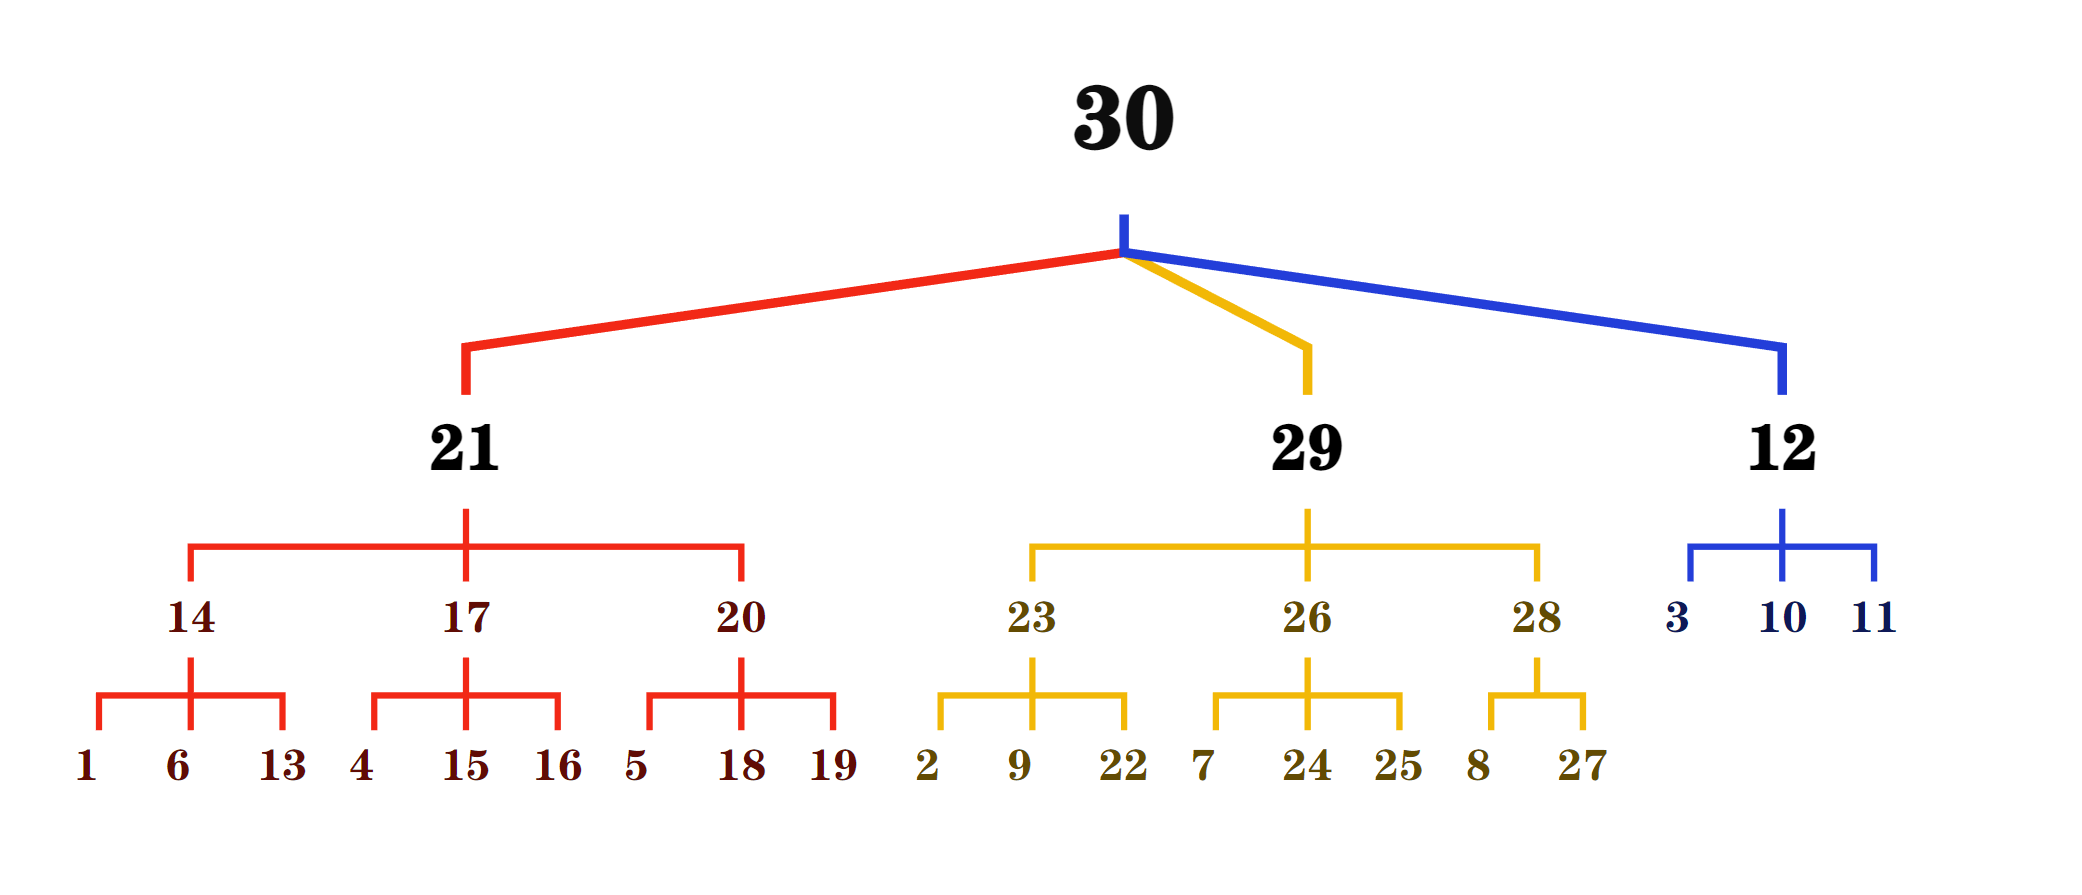
\includegraphics[width=0.8\textwidth]{result1}
    \caption{The heap after inserting a sequence ranging from 1 to 30}
\end{figure}

After performing the operation EXTRA-MAX, \textbf{the function return 30}. 
And the heap is as follows:
\begin{figure}[H]
    \centering  %图片全局居中
    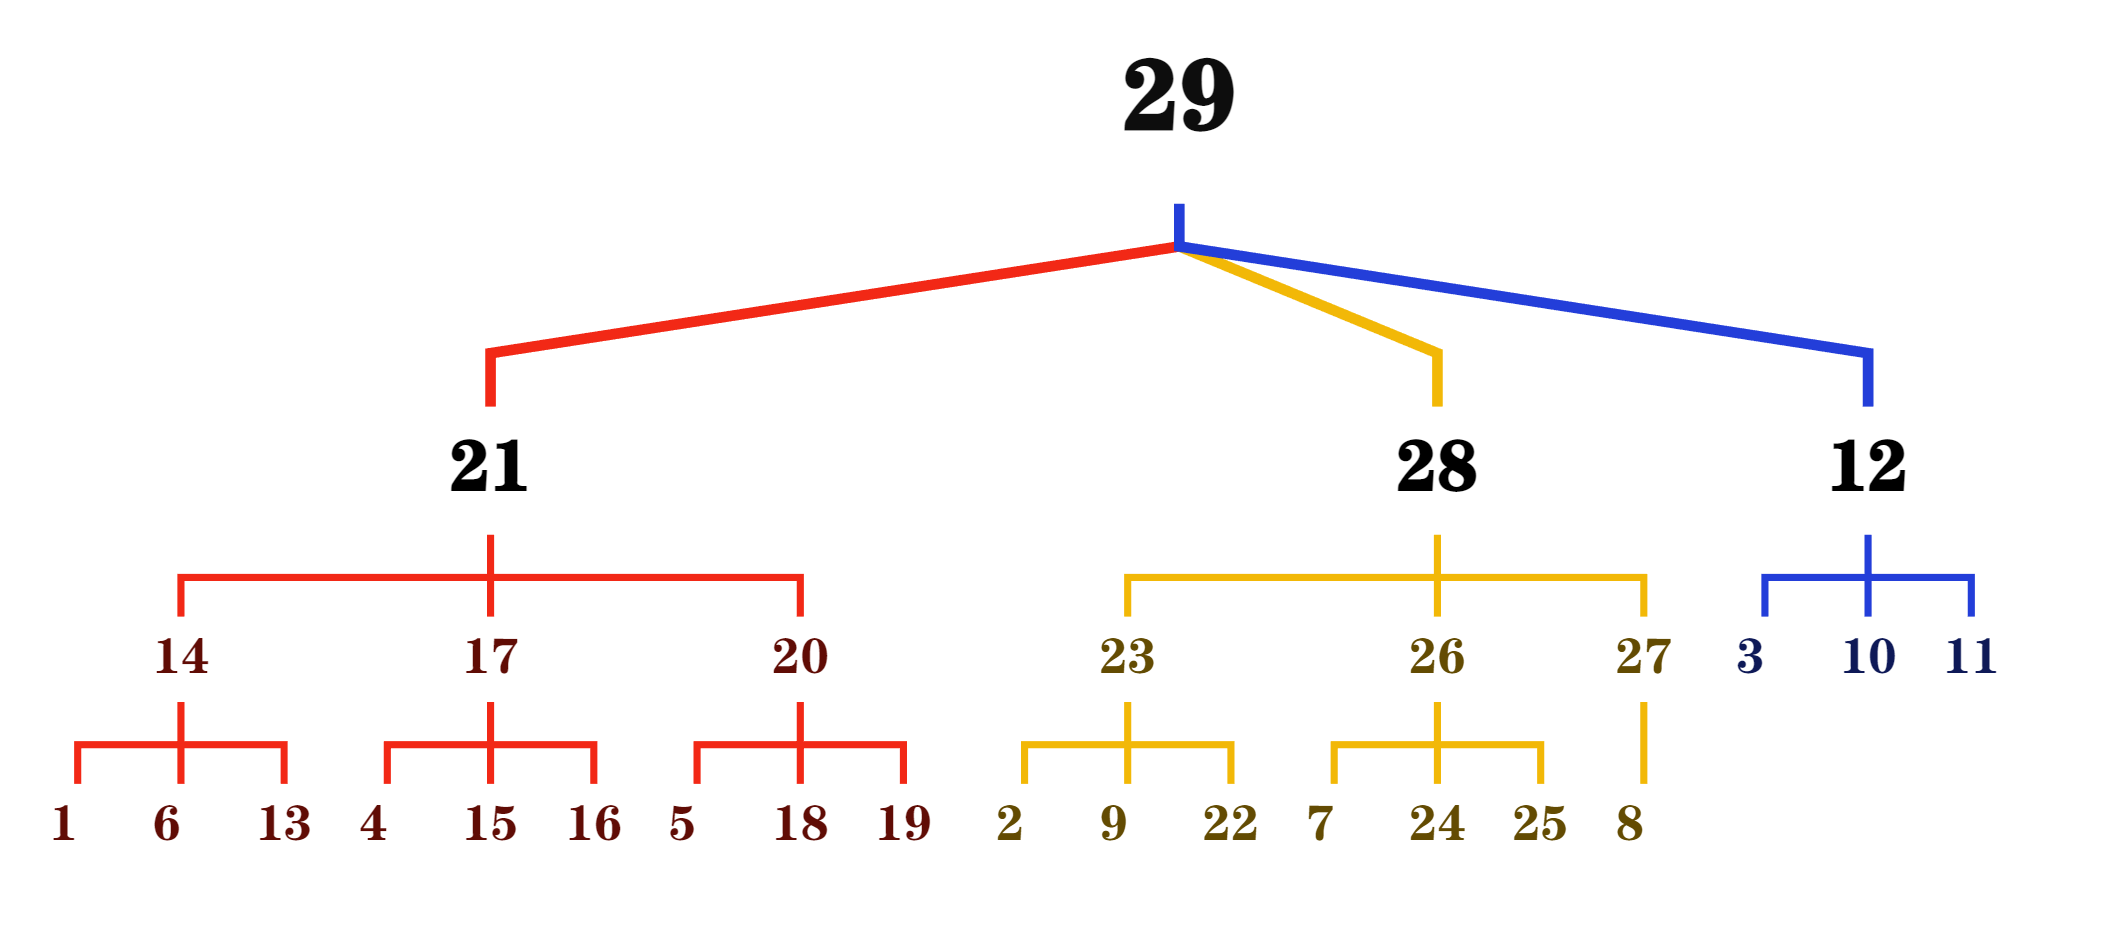
\includegraphics[width=0.8\textwidth]{result2}
    \caption{The heap after performing EXTRA-MAX}
\end{figure}

After performing the operation of INCREASE-KEY(A, 10, 28), the heap looks like:
\begin{figure}[H]
    \centering  %图片全局居中
    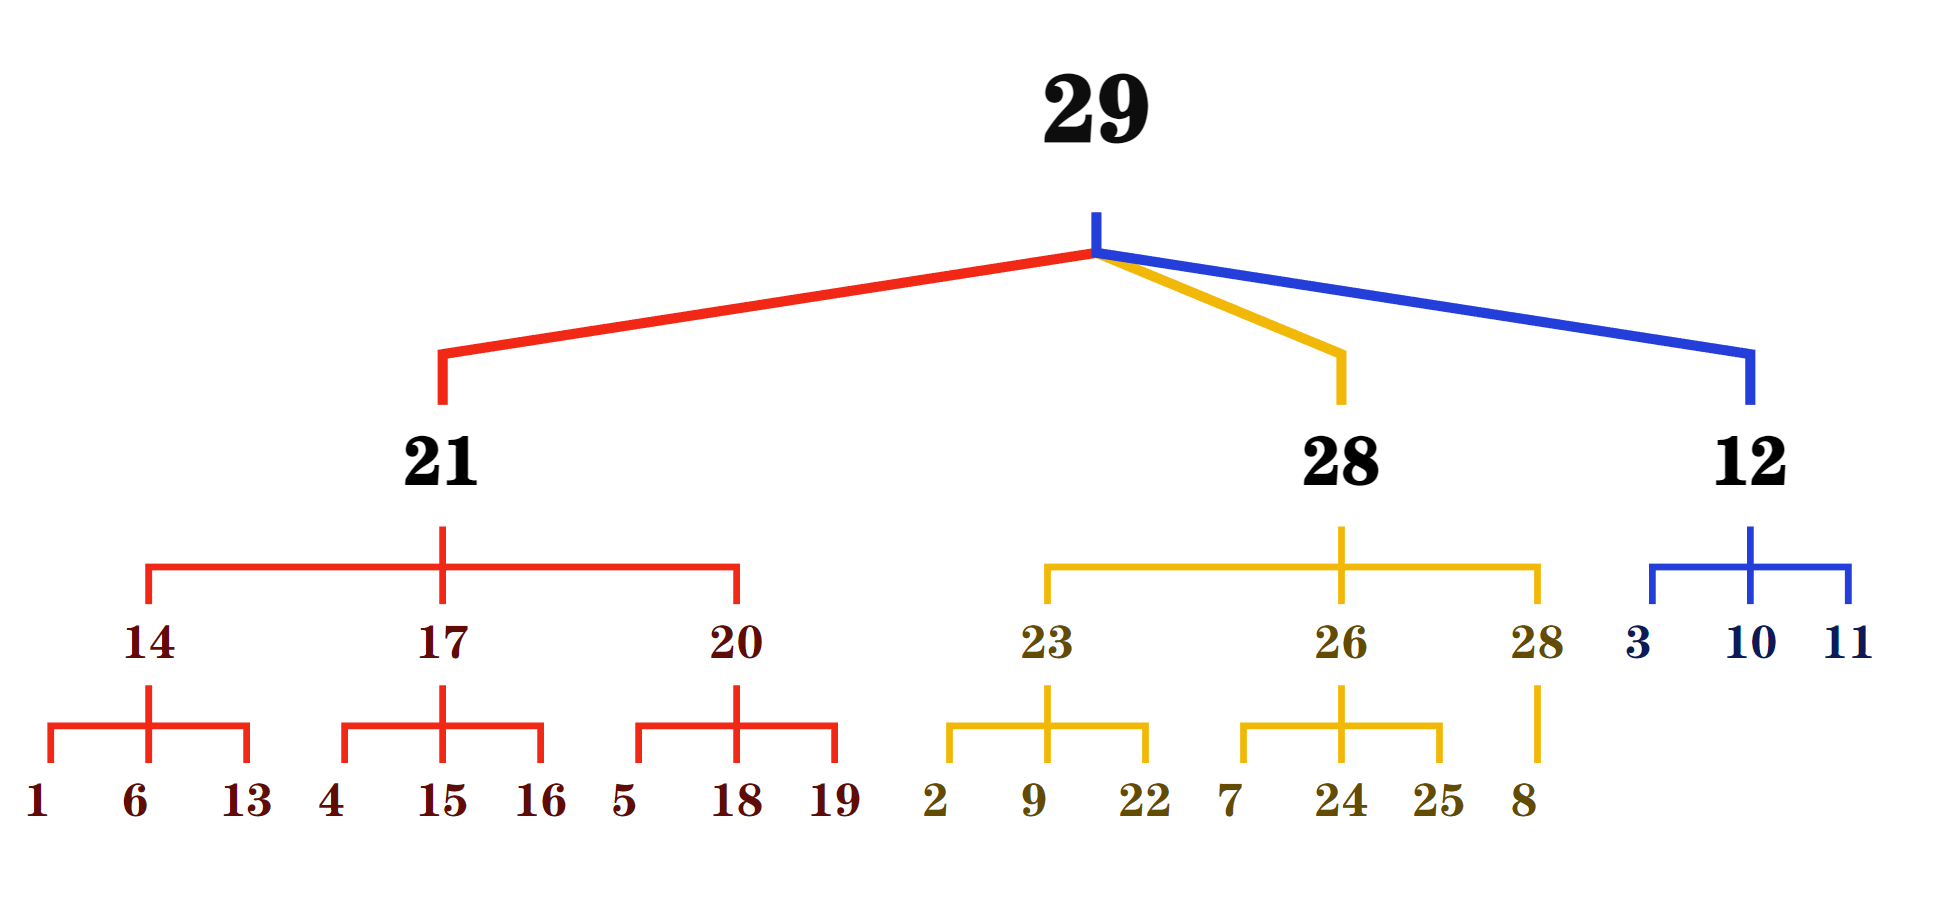
\includegraphics[width=0.8\textwidth]{result3}
    \caption{The heap after performing INCREASE-KEY(A, 10, 28)}
\end{figure}


\section*{Appendix: all of my python codes}
\lstinputlisting[style = Python,
caption={All of my python codes},
label = {increase-key}]{d_ary_heap.py} 

\end{document}